\documentclass{article}
\usepackage{amsmath,amsfonts,amssymb,graphicx,color,float}
\begin{document}
\section*{4 Filtering a time series with the designed filter}
\subsection*{\small 4.1 First iteration of the designed filter on a time series}
Filtering the time series with designed filter presented in chapter 2 has been performed with the statistical software R. The results of the filtering operation are represented in figure 11.
\begin{figure}[H]
  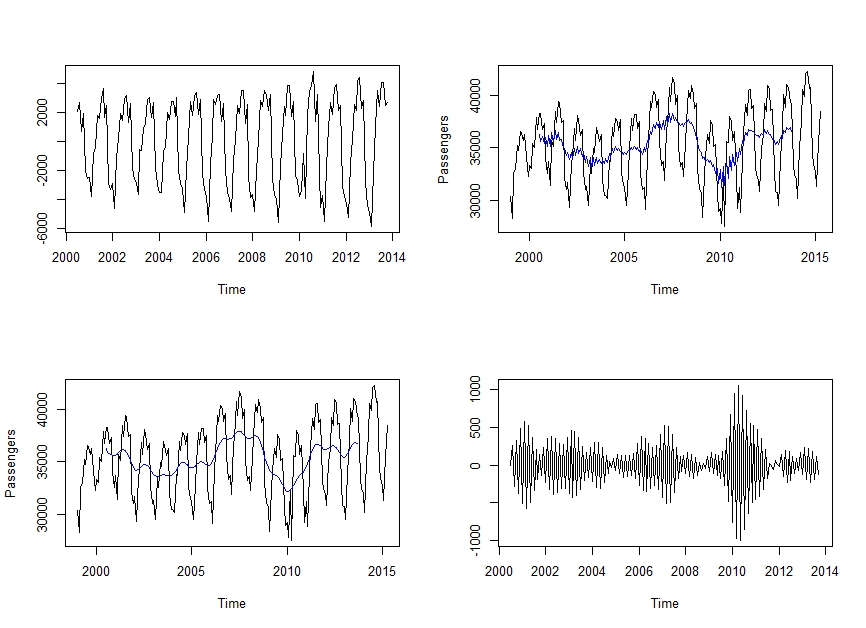
\includegraphics[width=\textwidth]{../images/capitolo4/collage.jpeg}
  {\textbf{\scriptsize Figure 11: Decomposition of the time series and comparison of designed filter with the most common ones.}}
\end{figure}
Top-left panel of figure 11 represents the seasonal component, obtained with a single iteration of the designed filter through the multiplication of formula 8. Then, this component has been subtracted from the original series, in order to obtain the \textit{trend+cycle+noise} series, represented in the top-right panel (blue line) in a comparison with the original data (black line). It is worth to highlight again that the sum of this \textit{trend+cycle+noise} and the seasonal factor is identical to the original time series. According to equation 14, it is then simple and straightforward to identify the high-frequency (noise) component and then to subtract it from this \textit{trend+cycle+noise} series. The pure smooth \textit{trend+cycle} component (the one in blue as well) is compared again to the original data (black line) in the bottom-left panel. At last, bottom-right chart reveals the high frequencies component, i.e. the ``noise'' of the series, which shows a strong increase in amplitude in the year 2010. Actually, an explanation of this increase could be that two of the additive outliers detected by both TRAMO/SEATS and X-13-ARIMA are in this year, at the months April and December.\\The outcome of the seasonally adjusted data is not totally satisfactory. While clearly a great deal of the seasonal pattern is removed, the visual impression is that the filtering has not been completely successful. One of the reasons for this is the strong amplitude of the seasonal component. One could deal with this in a number of ways; one possibility is simply to repeat the filtering process, but since the aim of this study is the analysis of the output of the seasonal adjustment procedures with the filtered series as input, the second filtering operation will be not performed in here. Figure 12 plots the JDemetra+ periodogram of the data filtered, through R, with the designed filter, before the performance of the further seasonal adjustment. This time, as opposed to what was done in chapter 3, there is no need for differencing the time series, since it is already stationary. Therefore, the first difference operation has been removed.\\ 
\begin{figure}[H]
\centering
  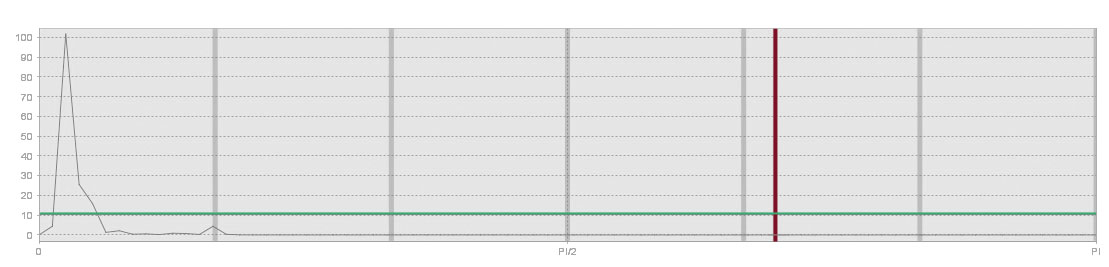
\includegraphics[width=\textwidth]{../images/capitolo4/tc_periodogram.jpg}
  {\textbf{\scriptsize Figure 12: Filtered time series periodogram.}}
\end{figure}
As proof of the imperfect seasonality removal, a peak is visible at the first seasonal frequency of 1/12 cycles/month. This imperfect removal after one pass of the filter is due to the fact that the frequency of 1/12 cycles/month is near the edge of the band which the seasonal filter removes. The removal is therefore slightly less than 100\%, which will leave a noticeable residual for a signal with a very strong annual variation. One could try to deal with this by making the band to be removed slightly broader, but this would imply that there would also be some undesirable suppression of genuine longer term cycle behavior. Another option might be to try and produce a sharper transition in the band-pass filter from the region in the spectrum where it passes all signal to the region in the spectrum where all signals are blocked. While this is possible, the effect this has is that in the time domain the linear coefficients of the filter function are non-zero over a larger range. In practice there is always a trade-off between the level to which seasonal behaviour can be suppressed in the time series for trend+cycle+noise, and the range over which the filter function has non-zero values. Apart from this limitation, the periodogram has values equal to zero for all the frequencies after the first seasonal one. It means that the removal of the seasonal component through the designed filter works properly at all the other harmonics. As a confirmation of the efficient seasonal removal, it is possible to compare this periodogram and the one in figure 8 and 9, of the seasonally adjusted series obtained through TRAMO/SEATS and X-13-ARIMA.\\
\subsection*{\small 4.2 Filtered series as input for JDemetra+ analysis}
The filtered time series (the \textit{trend+cycle} series represented in bottom-left chart of figure 11 ) has been used as input for a JDemetra+ analysis. On some occasions, TRAMO provides a not decomposable model. It happens when components have a negative spectrum for some frequencies. It is then said that the model presents a “non-admissible” decomposition. When this happens, SEATS automatically modifies the model parameters, searching for a decomposable model that is not far from the TRAMO one. The search always converges. For a more extensive discussion, see Maravall (2008). This is the case of the TRAMO analysis performed on the filtered series, which finds the as model not decomposable.\\ {\color{green}The original models identified by X-13-ARIMA and TRAMO/SEATS are both ARIMA models (3,2,1) (0,1,1). As previously specified, the analysis considers only so-called airline models, so the parameters have been replaced with the values (0,1,1) (0,1,1). The original high autoregressive parameter number (three) means the need to correct problem of autocorrelation results.} Before comparing the spectral analysis of the outputs, it is worth to compare the seasonal components obtained from the decomposition performed on the filtered data and on the non-filtered data.
\begin{figure}[H]
    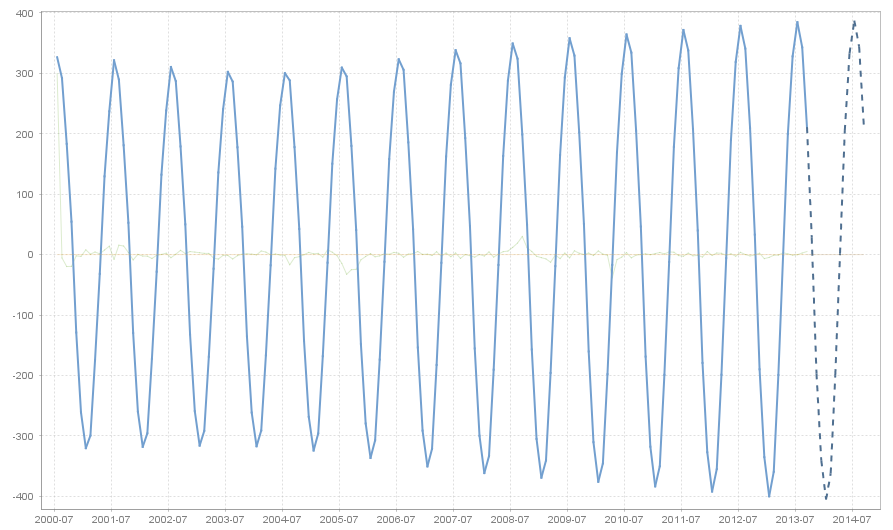
\includegraphics[width=\textwidth]{../images/capitolo4/X13_seas_cmp_filtered.jpg}
\end{figure}
\begin{figure}[H]
    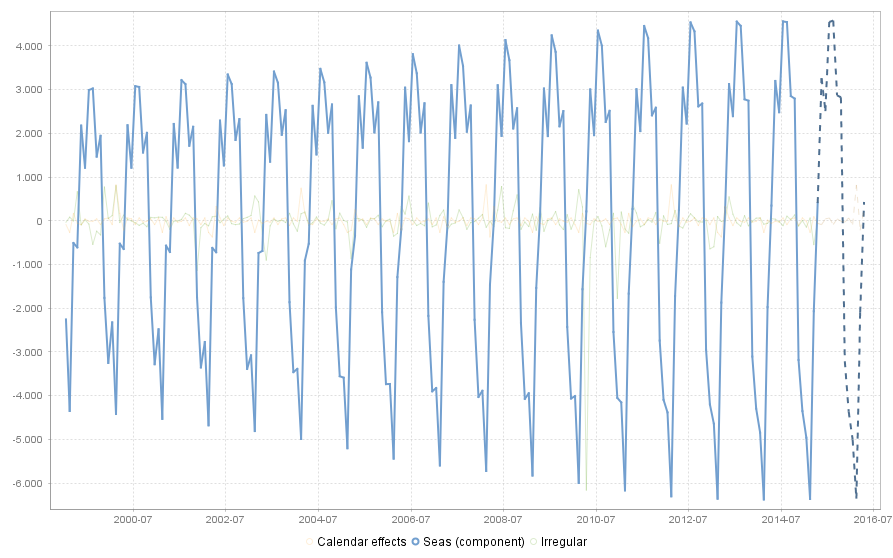
\includegraphics[width=\textwidth]{../images/capitolo4/X13_seas_cmp_plan.jpg}
      {\textbf{\scriptsize Figure 13: Comparison of seasonal factors obtained through X-13-ARIMA decomposition (TRAMO/SEATS acts similar). To the left is the filtered data seasonal component, to the right the non-filtered data seasonal component.}}
  \end{figure}
Relevant is the difference in the amplitude of the seasonal factor. The right chart, of the not filtered data, shows an amplitude ranging between -6000 and 4000. The seasonal factor component of the filtered data (on the left) shows a trend either smoother (at the peaks) and lower, ranging between -400 and 400.\\In the following charts are presented the spectral diagnostics of the outputs of the TRAMO/SEATS method, obtained when using the filtered series as input
\begin{figure}[H]
  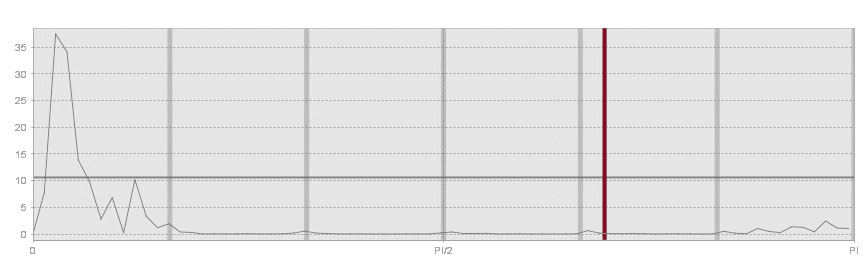
\includegraphics[width=\textwidth]{../images/capitolo4/TSresper.jpg}
\end{figure}
\begin{figure}[H]
  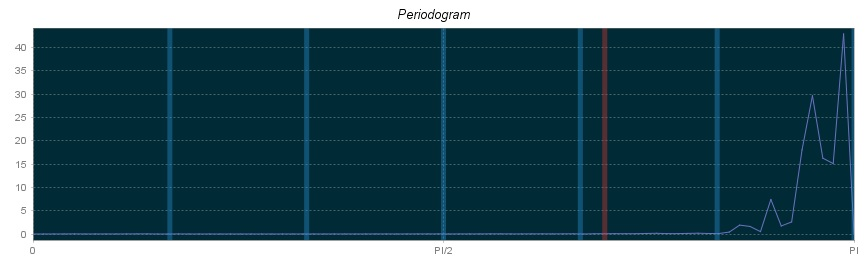
\includegraphics[width=\textwidth]{../images/capitolo4/TSirrper.jpg}
\end{figure} 
\begin{figure}[H]
  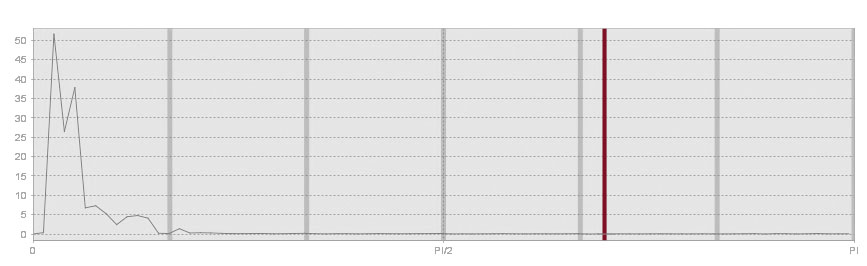
\includegraphics[width=\textwidth]{../images/capitolo4/TSsaper.jpg}
  {\textbf{\scriptsize Figure 14: Residuals, Irregular and seasonal adjusted periodogram obtained by TRAMO/SEATS.}}
\end{figure}
Most relevant result about these periodograms is the total absence of power at any seasonal frequency. This is a proof of the efficacy of the designed filter, particularly when the filtered series is used as input for further analysis. The comparison between figure 14 and the periodograms analyzed in chapter 3 confirms this latter statement. Periodograms obtained from X-13-ARIMA shows a similar behaviour to the TRAMO/SEATS ones, and therefore they will not be reported in here.\\JDemetra+ offers many diagnostics. Some of them are related to the presence of seasonality. As proof of the removal of the seasonal component, table 3 represents the results of those tests (for both the procedures), whose check for the presence of seasonality in the seasonally adjusted series. An explanation of these test is offered by Grudkowska (2015). As desirable, the response of these test testifies the efficient removal of the seasonal factor from the time series.
\begin{figure}[H]
  \begin{minipage}[b]{0.5\textwidth}
    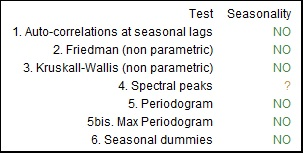
\includegraphics[width=\textwidth]{../images/capitolo4/testTS.jpg}
  \end{minipage}
  \hfill
  \begin{minipage}[b]{0.5\textwidth}
    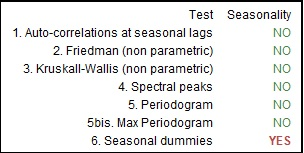
\includegraphics[width=\textwidth]{../images/capitolo4/testX13.jpg}
  \end{minipage}
  {\textbf{\scriptsize Table 3: JDemetra+ output for seasonality test on seasonally adjusted series; TRAMO/SEATS on the left and X-13-ARIMA on the right.}}
\end{figure}
When fitting a model to a time series, one of the most reliable indicator of the goodness of the fit is the Akaike information criterion (Akaike, 1974). When choosing between two different models, it is preferable to use the one with the lowest AIC value. This value in the two X-13-ARIMA procedures (the first for the original data, the second for the filtered data) is significantly different: respectively 2842.46 for the original time series and 1761.82 for the filtered time series.\\At last, figure 15 shows the squared gain of the components filters used by TRAMO/SEATS for the filtered time series decomposition. It is perfectly visible that the square gain of the seasonally adjusted filter catches much more signal if compared to the one of the original data, visible at figure 10, for it has value equal to one between the seasonal frequencies. It means that the seasonal component of the filtered data is much more deterministic than the one of the original data. As proof of this, the bright blue line, related to the seasonal factor filter, has value equal to zero for all the frequencies out of the seasonal ones. Furthermore, the squared gain of the trend filter has higher values at all the frequencies respect to the one of figure 10. It means that all information about long term behavior is delivered to the output series.
\begin{figure}[H]
  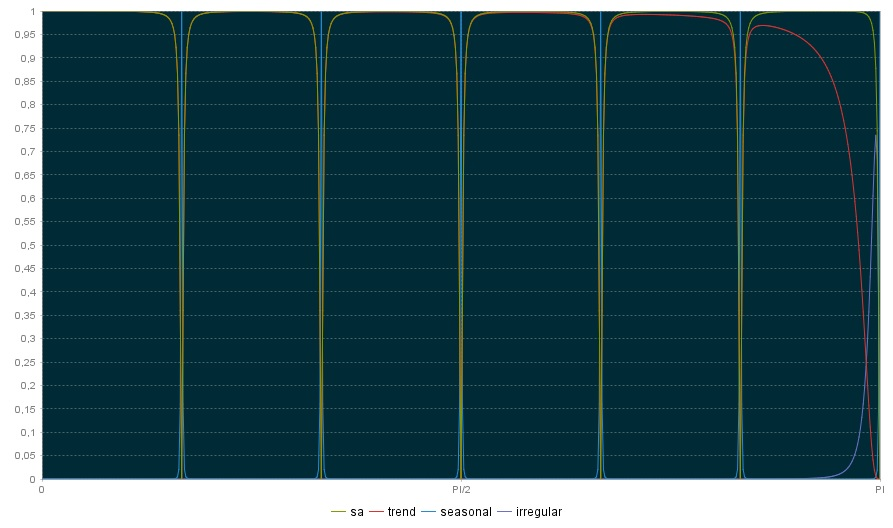
\includegraphics[width=\textwidth]{../images/capitolo4/gainfilters.jpg}
  {\textbf{\scriptsize Figure 15: Gain filter of the components of TRAMO/SEATS procedure applied to filtered time series.}}
\end{figure}
\end{document}